\section{Stoke's Theorem and Divergence Theorem}

In this lab you will study the properties of the vector field
%
\begin{equation}
\label{eq:theVectorField}
\vec{v} = \frac{1}{\sqrt{0.2 + y^4 - 2xy^2 + x^2 + x^4 - 2x^2y + y^2}} \left[ \left(-y^2 + x \right) \hat{i} + \left( x^2 - y \right) \hat{j} + 0 \hat{k} \right]
\end{equation}
%
in the ranges $-2 < x < 2$, $-2 < y < 2$, $-2 < z < 2$ using Mathematica.
Begin by clearing any existing variables, defining the function, and defining variable ranges:
%
\begin{verbatim}
ClearAll["Global`*"];
denom[x_, y_] = Sqrt[0.2 + y^4 - 2*x*y^2 + x^2 + x^4 - 2*x^2*y + y^2];
vx[x_, y_] = (-y^2 + x)/denom[x, y];
vy[x_, y_] = (x^2 - y)/denom[x, y];
xmin = -2;
xmax = 2;
ymin = -2;
ymax = 2;
\end{verbatim}
%
Next, plot the vector field.
Since the field does not depend on $z$ and since the $z$-component is zero, a 2D plot will suffice.
Use VectorPlot and StreamPlot to get two different representations of the same function:
%
\begin{verbatim}
vp = VectorPlot[{vx[x, y], vy[x, y]}, {x, xmin, xmax}, {y, ymin, ymax}];
sp = StreamPlot[{vx[x, y], vy[x, y]}, {x, xmin, xmax}, {y, ymin, ymax}];
Grid[{{vp, sp}}]
\end{verbatim}
%
\begin{figure}[!h]
\centering
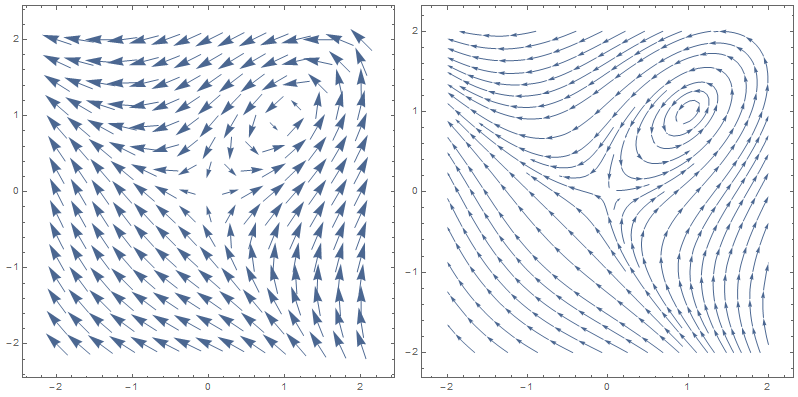
\includegraphics[scale=0.6]{figures/stokes-theorem/theVectorFieldPlots}
\caption{Plots of the vector field defined in equation~\ref{eq:theVectorField}.}
\label{fig:theVectorFieldPlots}
\end{figure}

\pagebreak

%%%%%%%%%%%%%%%%%%%%%%%%%%%%%%%%%%%%%%%%%%%
%%%%%%%%%%%%%%%%%%%%%%%%%%%%%%%%%%%%%%%%%%%

\underline{Part 1 - Stoke's Theorem}
\hfill \break

Stoke's Theorem states
%
\begin{equation}
\label{eq:stokesTheorem}
\oint_{Path} \vec{v} \cdot d\vec{s} = \int_{Surface} \left( \nabla \times \vec{v} \right) \cdot d\vec{A}.
\end{equation}
%
In this example, since the $z$-component of the field is zero, and since the field does not depend on z, Stoke's Theorem can be simplified to
%
\begin{equation}
\label{eq:stokesTheoremSimplified}
\oint_{Path} \vec{v} \cdot d\vec{s} = \int_{Surface} \left( \nabla \times \vec{v} \right)_z dA.
\end{equation}
%
Use Mathematica to calculate the curl of $\vec{v}$ (i.e. $\nabla \times \vec{v}$) and print out a few values at random points:
\begin{verbatim}
curlv[x_, y_, z_] = Curl[{vx[x, y], vy[x, y], 0}, {x, y, z}]
curlv[1, 1, 0]
curlv[1, 1, 0][[3]]
\end{verbatim}
notice that the $x$ and $y$ components of the curl of this vector field are zero.
Now make a plot of $\left( \nabla \times \vec{v} \right)_z$ as a function of $x$ and $y$ (remember, it doesn't depend on $z$):
\begin{verbatim}
dpz = DensityPlot[curlv[x, y, 0][[3]], {x, xmin, xmax}, {y, ymin, ymax},
	PlotLegends -> Automatic]
\end{verbatim}
%
\begin{figure}[!h]
\centering
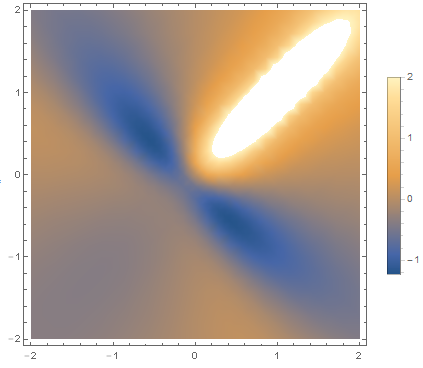
\includegraphics[scale=0.7]{figures/stokes-theorem/curlzDensityPlot.png}
\caption{$\left( \nabla \times \vec{v} \right)_z$}
\label{fig:curlzDensityPlot}
\end{figure}
%
and compare figures~\ref{fig:theVectorFieldPlots} and \ref{fig:curlzDensityPlot}.
Notice that the curl is large in the region where the field is ``curly.''

Create a grid in the $x$-$y$ plane and use a loop to get the value of the curl at the grid points:
\begin{verbatim}
nxdiv = 10;
nydiv = 10;
For[ix = 0, ix < nxdiv, ix++;
 For[iy = 0, iy < nydiv, iy++;
  xval = xmin + (ix - 0.5)*(xmax - xmin)/nxdiv;
  yval = ymin + (iy - 0.5)*(ymax - ymin)/nydiv;
  curlval = curlv[xval, yval, 0][[3]];
  vals = {xval, yval, curlval};
  Print[vals];
  ]] 
\end{verbatim}
and use these results to approximate the right hand side of equation~\ref{eq:stokesTheoremSimplified}.

Finally, use a similar technique to approximate the left hand side of equation~\ref{eq:stokesTheoremSimplified}.
For example:
\begin{verbatim}
(* ccw loop, starting at top right *)
nStepsPerSide = 20;
(* top: *)
For[i = 0, i < nStepsPerSide, i++;
 xval = xmax - (i - 0.5)*(xmax - xmin)/nxdiv;
 yval = ymax;
 vDotDs = vx[xval, yval]*(-1)*((xmax - xmin)/nStepsPerSide);
 Print[vDotDs];
 ]
(* left side: *)
For[i = 0, i < nStepsPerSide, i++;
 xval = xmin;
 yval = ymax - (i - 0.5)*(ymax - ymin)/nydiv;
 vDotDs = vy[xval, yval]*(-1)*((ymax - ymin)/nStepsPerSide);
 Print[vDotDs];
 ]
etc...
\end{verbatim}
Once your program is fully written and debugged, increase $nxdiv$, $nydiv$, and $nStepsPerSide$ to $100$ to improve your accuracy.
Confirm Stoke's Theorem by comparing your two calculated numbers.

%%%%%%%%%%%%%%%%%%%%%%%%%%%%%%%%%%%%%%%%%%%
%%%%%%%%%%%%%%%%%%%%%%%%%%%%%%%%%%%%%%%%%%%

\hfill \break
\underline{Extra Credit - The Divergence Theorem}
\hfill \break

Use a similar approach to confirm the Divergence Theorem for this same vector field.

\pagebreak \clearpage
